% On découpe ce document complexe en plusieurs sous-fichiers séparés.
% Cela permettra notamment de réarranger les transparents facilement 
% lors de l'élaboration du document.

% La définition de la classe beamer avec tous les styles afférents

\RequirePackage{currfile} 

\documentclass[xcolor=table]{beamer}
\usepackage{animate}
\usepackage{colortbl}

%%% Гиперссылки



%%%%%%%%%%%%%%%%%%%%%%%%%%%%%%%%%%%%%%%%%
% Beamer Presentation
% LaTeX Template
% Version 1.0 (10/11/12)
%
% This template has been downloaded from:
% http://www.LaTeXTemplates.com
%
% License:
% CC BY-NC-SA 3.0 (http://creativecommons.org/licenses/by-nc-sa/3.0/)
%
%%%%%%%%%%%%%%%%%%%%%%%%%%%%%%%%%%%%%%%%%

%----------------------------------------------------------------------------------------
%	PACKAGES AND THEMES
%----------------------------------------------------------------------------------------




\mode<presentation> {

% The Beamer class comes with a number of default slide themes
% which change the colors and layouts of slides. Below this is a list
% of all the themes, uncomment each in turn to see what they look like.

%\usetheme{default}
%\usetheme{AnnArbor}
%\usetheme{Antibes}
%\usetheme{Bergen}
%\usetheme{Berkeley}
%\usetheme{Berlin}
%\usetheme{Boadilla}
%\usetheme{CambridgeUS}
%\usetheme{Copenhagen}
%\usetheme{Darmstadt}
%\usetheme{Dresden}
%\usetheme{Frankfurt}
%\usetheme{Goettingen}
%\usetheme{Hannover}
%\usetheme{Ilmenau}
%\usetheme{JuanLesPins}
%\usetheme{Luebeck}
%\usetheme{Madrid}		
%\usetheme{Malmoe}
%\usetheme{Marburg}
%\usetheme{Montpellier}
%\usetheme{PaloAlto}
%\usetheme{Pittsburgh}
%\usetheme{Rochester}
%\usetheme{Singapore}
%\usetheme{Szeged}
\usetheme{Warsaw}

% As well as themes, the Beamer class has a number of color themes
% for any slide theme. Uncomment each of these in turn to see how it
% changes the colors of your current slide theme.

%\usecolortheme{albatross}
%\usecolortheme{beaver}
%\usecolortheme{beetle}
%\usecolortheme{crane}
%\usecolortheme{dolphin}
%\usecolortheme{dove}
%\usecolortheme{fly}
%\usecolortheme{lily}
%\usecolortheme{orchid}
%\usecolortheme{rose}
%\usecolortheme{seagull}
%\usecolortheme{seahorse}
\usecolortheme{whale}
%\usecolortheme{wolverine}

%\setbeamertemplate{footline} % To remove the footer line in all slides uncomment this line
%\setbeamertemplate{footline}[frame number] % To replace the footer line in all slides with a simple slide count uncomment this line

%\setbeamertemplate{navigation symbols}{} % To remove the navigation symbols from the bottom of all slides uncomment this line

\setbeamercovered{transparent} % Fait apparaître les animations en grisé (utile pour la conception, mais peut être commenté lors de la remise du document final)

% Pour utiliser une police à empattements partout
\usefonttheme{serif}

% Pour rajouter la numérotation des frames dans les pieds de page
\newcommand*\oldmacro{}%
\let\oldmacro\insertshorttitle%
\renewcommand*\insertshorttitle{%
  \oldmacro\hfill%
  \insertframenumber\,/\,\inserttotalframenumber}

}

\usepackage{graphicx} % Allows including images
\usepackage{booktabs} % Allows the use of \toprule, \midrule and \bottomrule in tables




% Les autres packages utiles  notamment pour le français, les accents ou Python
\usepackage{natbib}         % Pour la bibliographie
\usepackage{url}            % Pour citer les adresses web
\usepackage[T1]{fontenc}    % Encodage des accents
\usepackage[utf8]{inputenc} % Lui aussi
\usepackage[frenchb]{babel} % Pour la traduction française
\usepackage{numprint}       % Histoire que les chiffres soient bien

\usepackage{amsmath}        % La base pour les maths
\usepackage{mathrsfs}       % Quelques symboles supplémentaires
\usepackage{amssymb}        % encore des symboles.
\usepackage{amsfonts}       % Des fontes, eg pour \mathbb.

\usepackage{cancel}

%\usepackage[svgnames]{xcolor} % De la couleur

%%% Si jamais vous voulez changer de police: décommentez les trois 
%\usepackage{tgpagella}
%\usepackage{tgadventor}
%\usepackage{inconsolata}

%%% Pour L'utilisation de Python
\usepackage{minted}
\usemintedstyle{friendly}

\usepackage{graphicx} % inclusion des graphiques
\usepackage{wrapfig}  % Dessins dans le texte.

\usepackage{tikz}     % Un package pour les dessins (utilisé pour l'environnement {code})
\usepackage[framemethod=TikZ]{mdframed}

% Les macros et raccourcis personnels
% Ce fichier contient toutes les macros que vous pouvez avoir envie de définir 
% si vous les utilisez plusieurs fois dans le document.

\PassOptionsToPackage{svgnames}{color}

% Un environnement pour bien présenter le code informatique
\newenvironment{code}{%
\begin{mdframed}[linecolor=green,innerrightmargin=30pt,innerleftmargin=30pt,
backgroundcolor=black!5,
skipabove=10pt,skipbelow=10pt,roundcorner=5pt,
splitbottomskip=6pt,splittopskip=12pt]
}{%
\end{mdframed}
}

% Un raccourci pour composer les unités correctement (en droit)
% Exemple: $v = 10\U{m.s^{-1}}$
\newcommand{\U}[1]{~\mathrm{#1}}

% Les guillemets \ofg{par exemple}
\newcommand{\ofg}[1]{\og{}#1\fg{}}

% Le d des dérivées doit être droit: \frac{\dd x}{\dd t}
\newcommand{\dd}{\text{d}}

% La dérivée temporelle, tellement courante en physique, avec les d droits
\newcommand{\ddt}[1]{\frac{\dd #1}{\dd t}}

% Des parenthèses, crochets et accolades qui s'adaptent automatiquement à la 
% taille de ce qu'il y a dedans
\newcommand{\pa}[1]{\left(#1\right)}
\newcommand{\pac}[1]{\left[#1\right]}
\newcommand{\paa}[1]{\left\{#1\right\}}

% Un raccourci pour écrire une constante
\newcommand{\cte}{\text{C}^{\text{te}}}

% Pour faire des indices en mode texte (comme les énergie potentielles)
\newcommand{\e}[1]{_{\text{#1}}}

% Le produit vectoriel a un nom bizarre:
\newcommand{\vectoriel}{\wedge}


% On définit le titre et l'auteur du document

% L'argument optionnel (entre crochets) donne le titre qui sera mis sur chaque slide
\title[Meta-learning for model selection]{The principle of meta-learning for model selection in time series forecasting}
\author{Zekhov Matvei\\
\and Boris Demeshev}
% Votre nom
% L'épreuve (car on n'a pas le droit de signaler sa provenance à un concours) (là encore, l'argument optionnel apparaît sur chaque slide)
\institute[HSE]{Higher School of Economics}
\date{Session 2019} 

% On démarre le document proprement dit
\begin{document}

% La page de titre et la table des matières
% Rien d'autre à faire qu'afficher le titre
\begin{frame}
\titlepage 
\end{frame}

\begin{frame}
\frametitle{Model selection algorythm}

\begin{center}
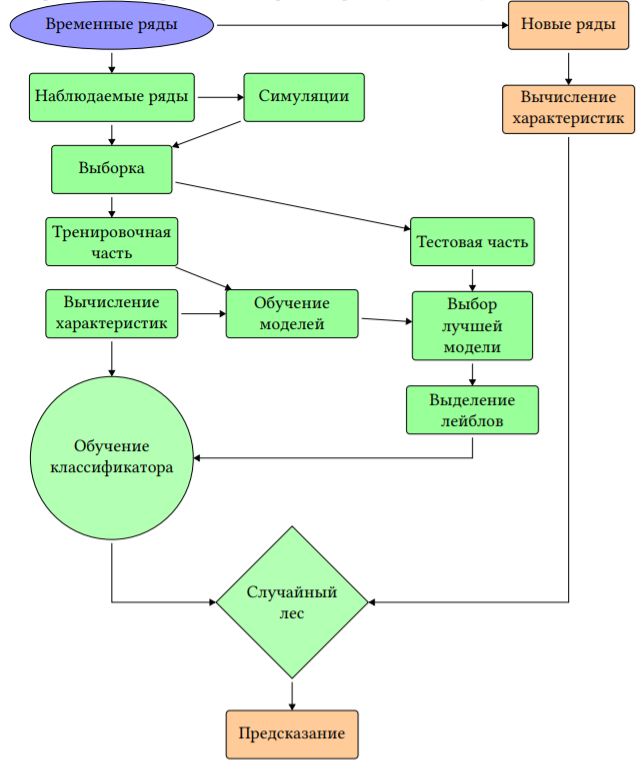
\includegraphics[width = 0.5\linewidth]{slides/graph.PNG}
\end{center}
\end{frame}

\begin{frame}
\frametitle{Sample}

\begin{table}[]
\resizebox{\textwidth}{!}{%
\begin{tabular}{|
>{\columncolor[HTML]{91FF91}}l |l|l|l|}
\hline
\textbf{Class} & \cellcolor[HTML]{91FF91}\textbf{Quantity} & \cellcolor[HTML]{91FF91}\textbf{Length} & \cellcolor[HTML]{91FF91}\textbf{Seasonality} \\ \hline
Yearly & 2000 & 30 & 1 \\ \hline
Quarterly & 2000 & 60 & 4 \\ \hline
Monthly & 2000 & 156 & 12 \\ \hline
Weekly & 286 & 315 & 4 \\ \hline
Daily & 2000 & 500 & 7 \\ \hline
Hourly & 245 & 720 & 24 \\ \hline
Total8531 &  &  &  \\ \hline
\end{tabular}%
}
\end{table}
\end{frame}

\begin{frame}
\frametitle{Time series exapmples}

\begin{center}
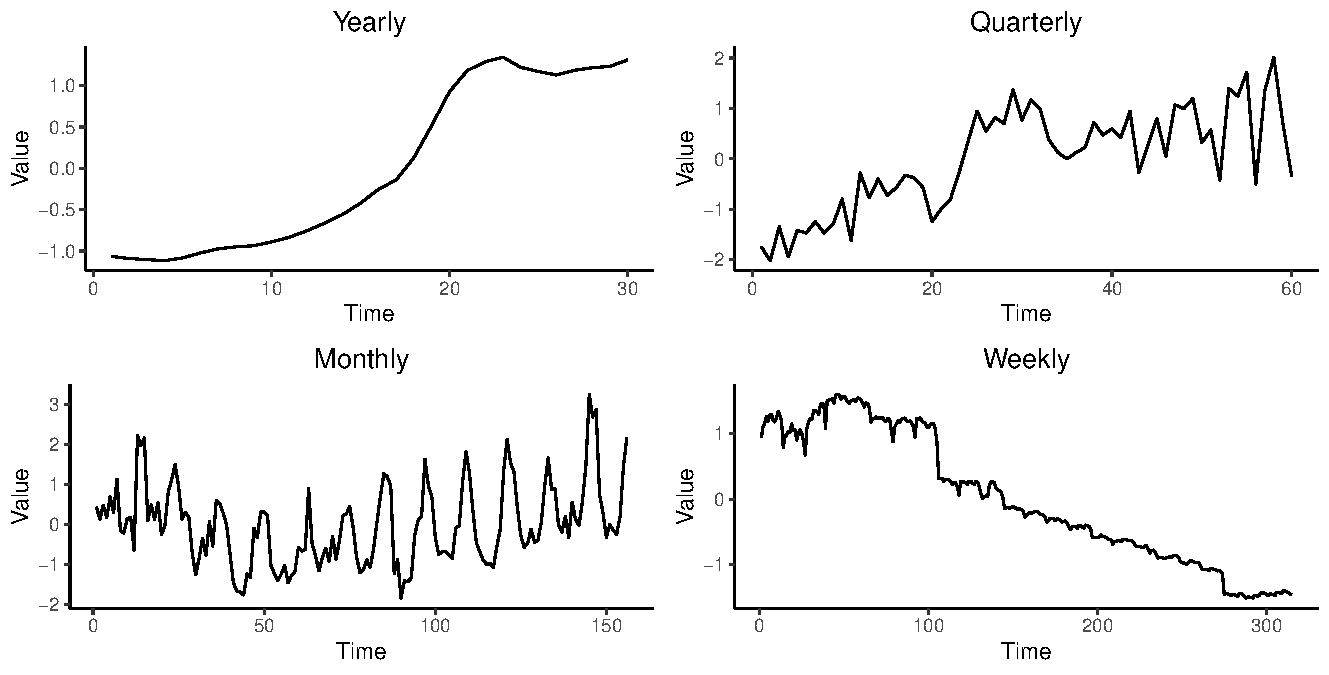
\includegraphics[width = \linewidth]{slides/time_series.pdf}
\end{center}
\end{frame}

\begin{frame}
\frametitle{Correlation of features}

\begin{center}
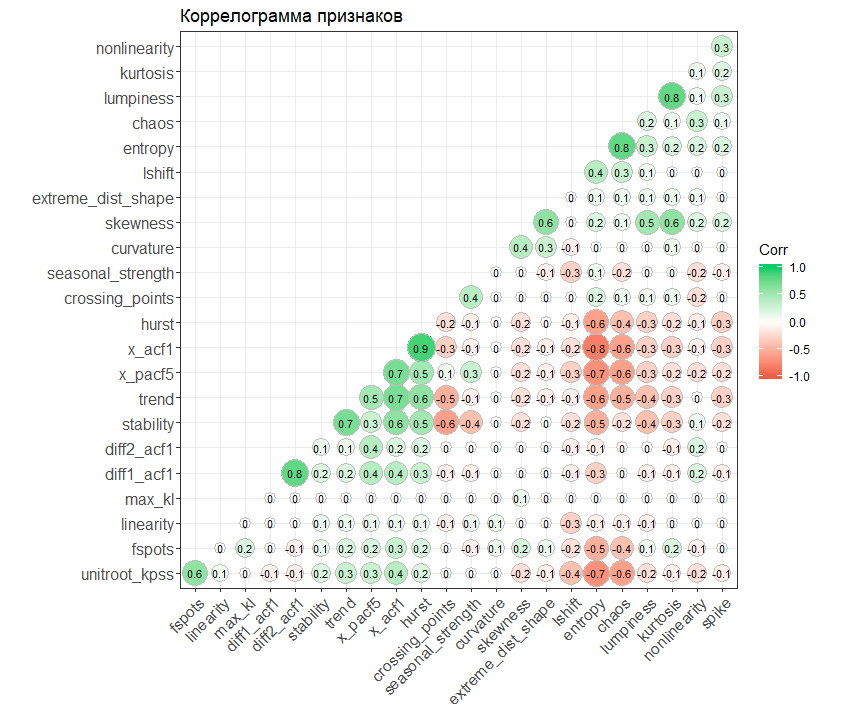
\includegraphics[width = 0.8\linewidth]{slides/corr.png}
\end{center}
\end{frame}

\begin{frame}
\frametitle{UMAP embeddings}

\begin{center}
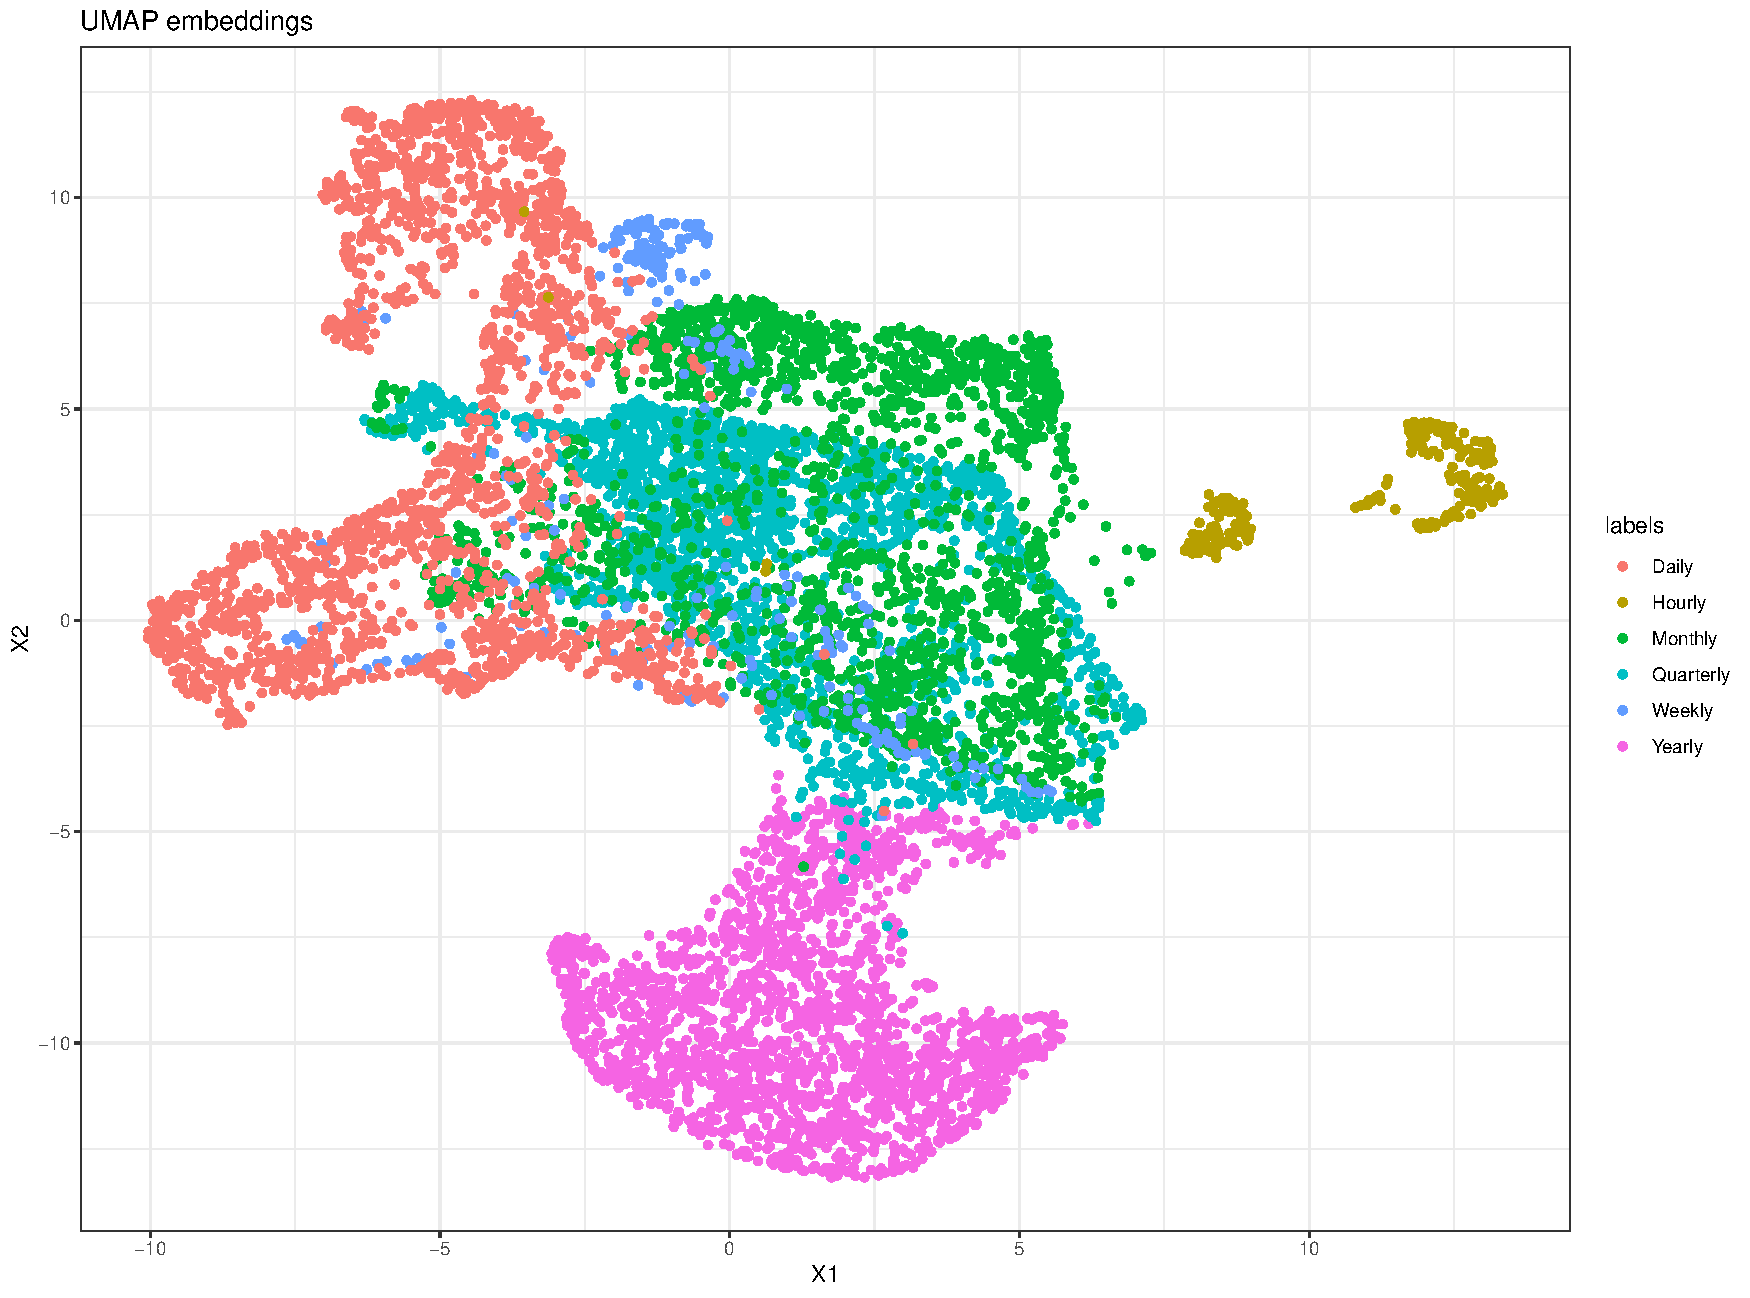
\includegraphics[width = \linewidth]{slides/umap.pdf}
\end{center}
\end{frame}


\begin{frame}
\frametitle{PCA}

\begin{center}
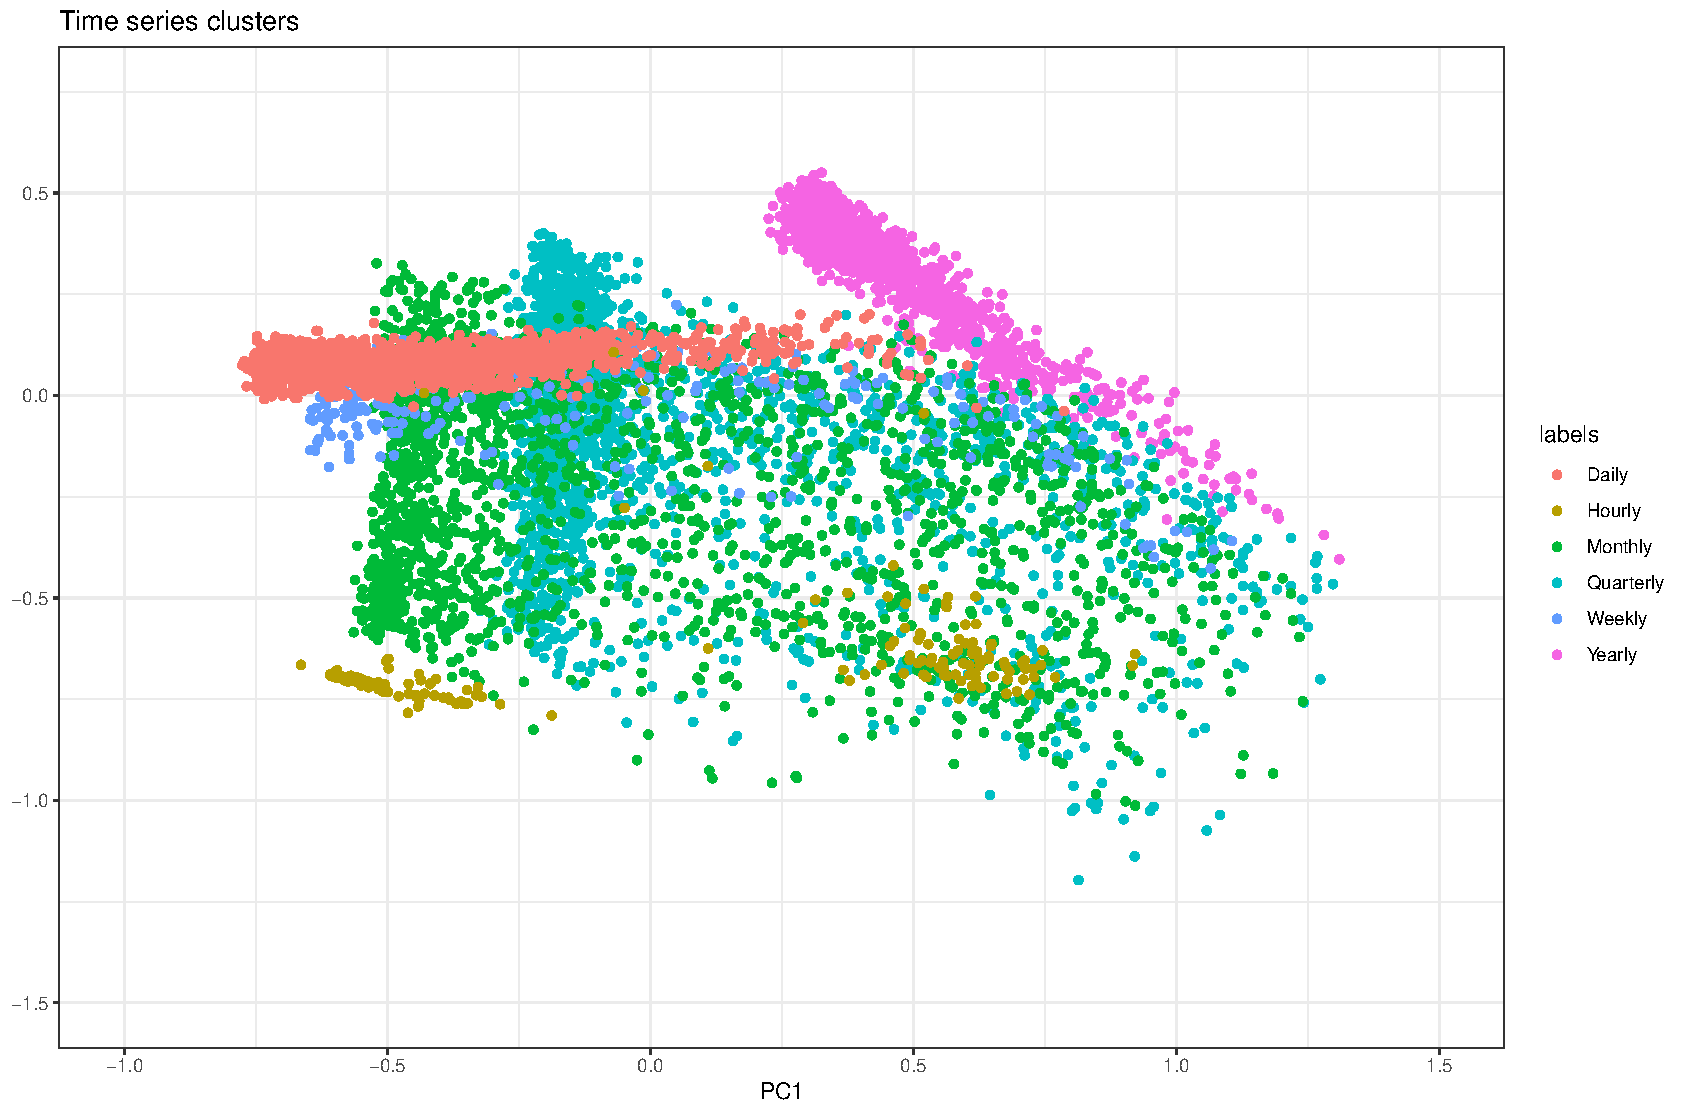
\includegraphics[width = \linewidth]{slides/pca.pdf}
\end{center}
\end{frame}


\begin{frame}
\frametitle{Strength of features}

\begin{center}
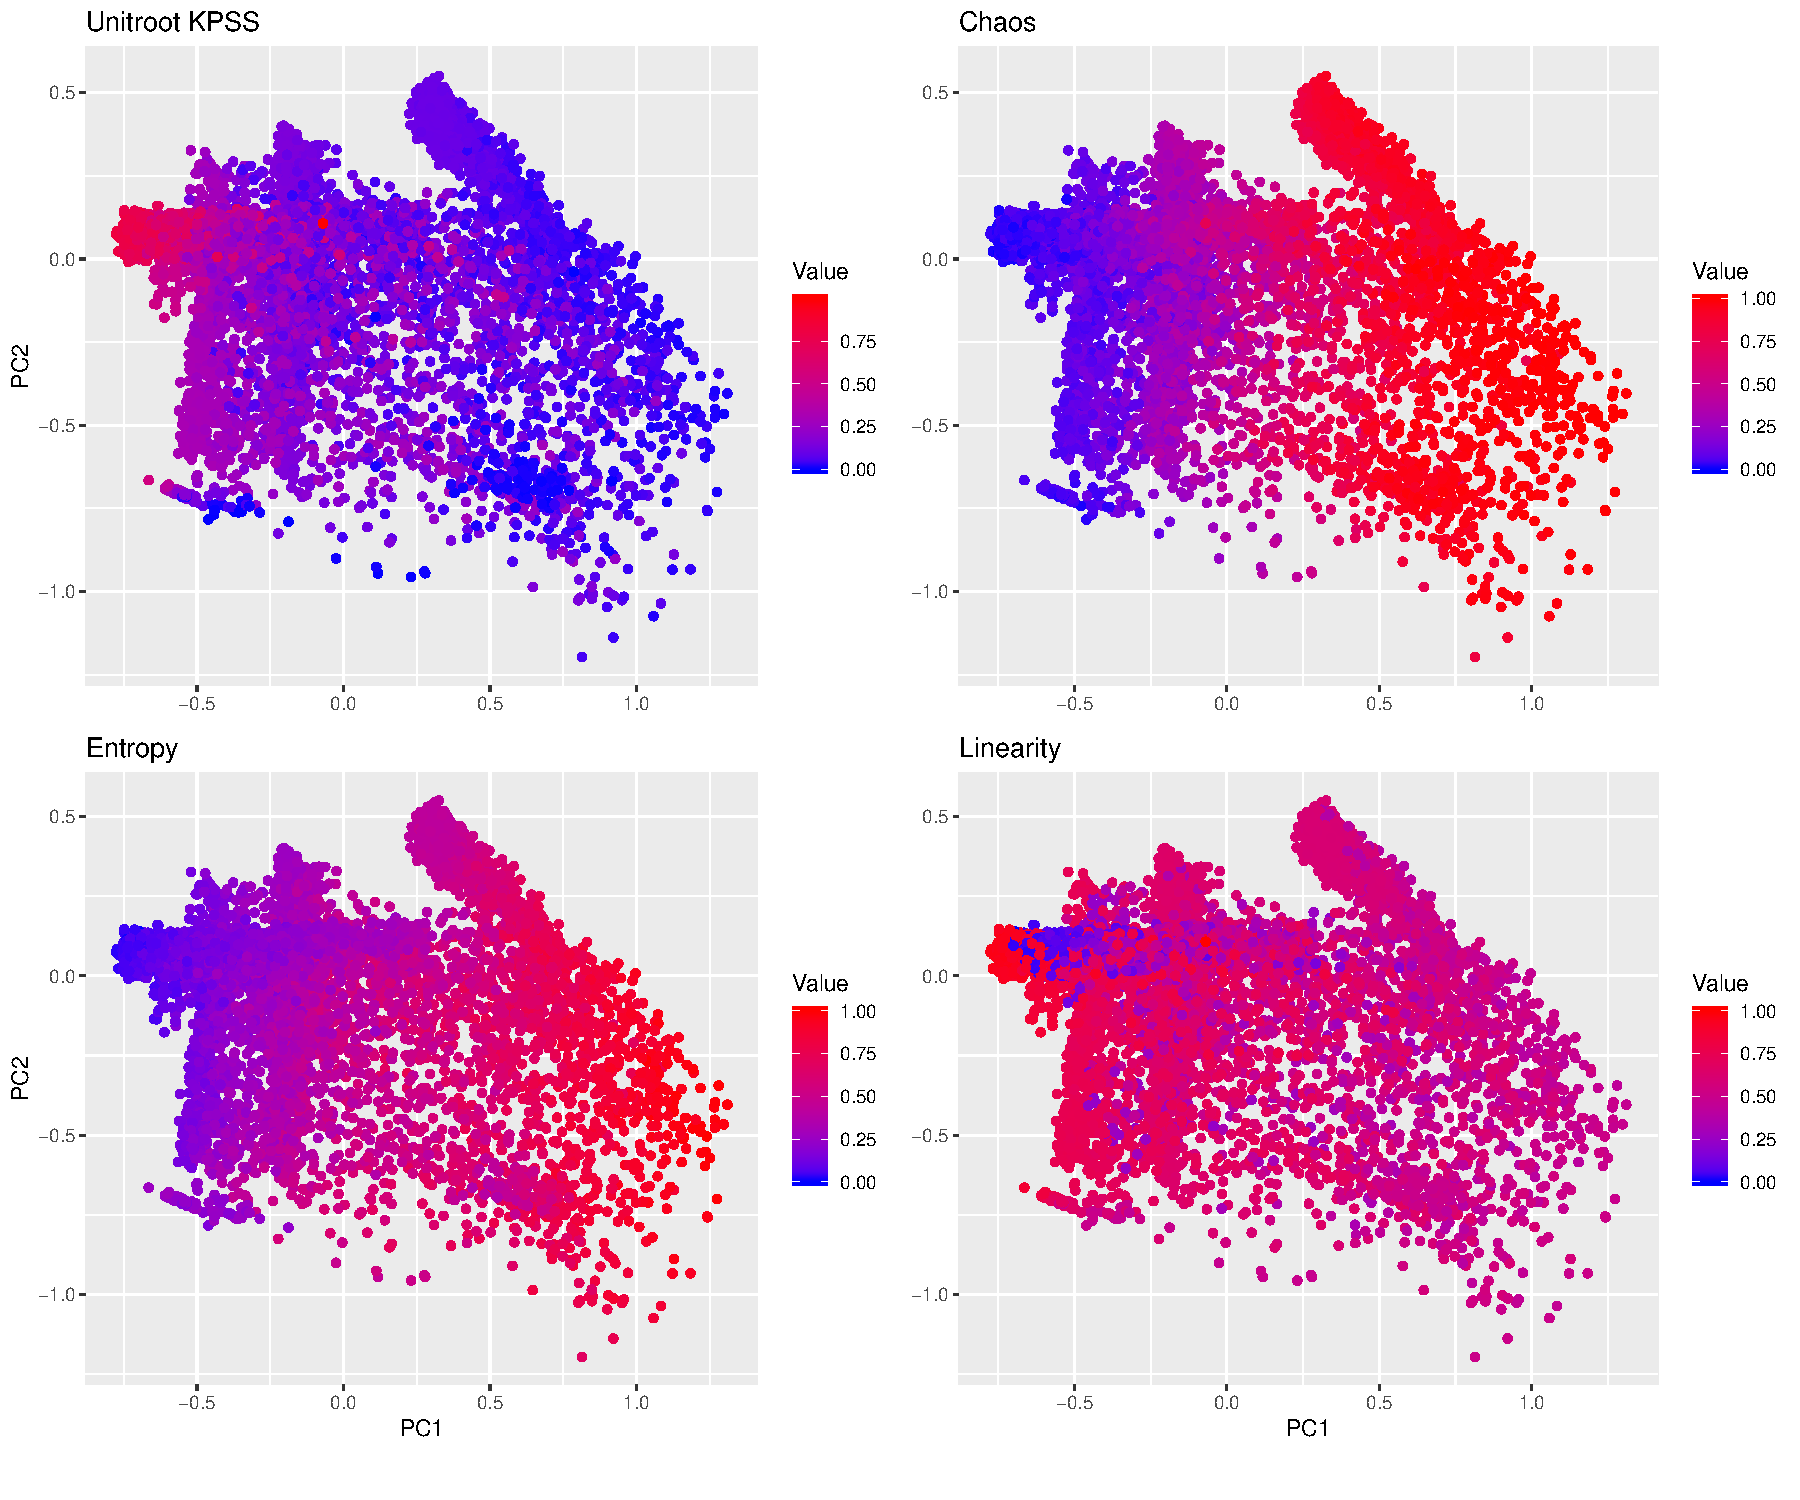
\includegraphics[width = 0.8\linewidth]{slides/fin_str.pdf}
\end{center}
\end{frame}




\begin{frame}
\frametitle{New series generation}

\begin{center}
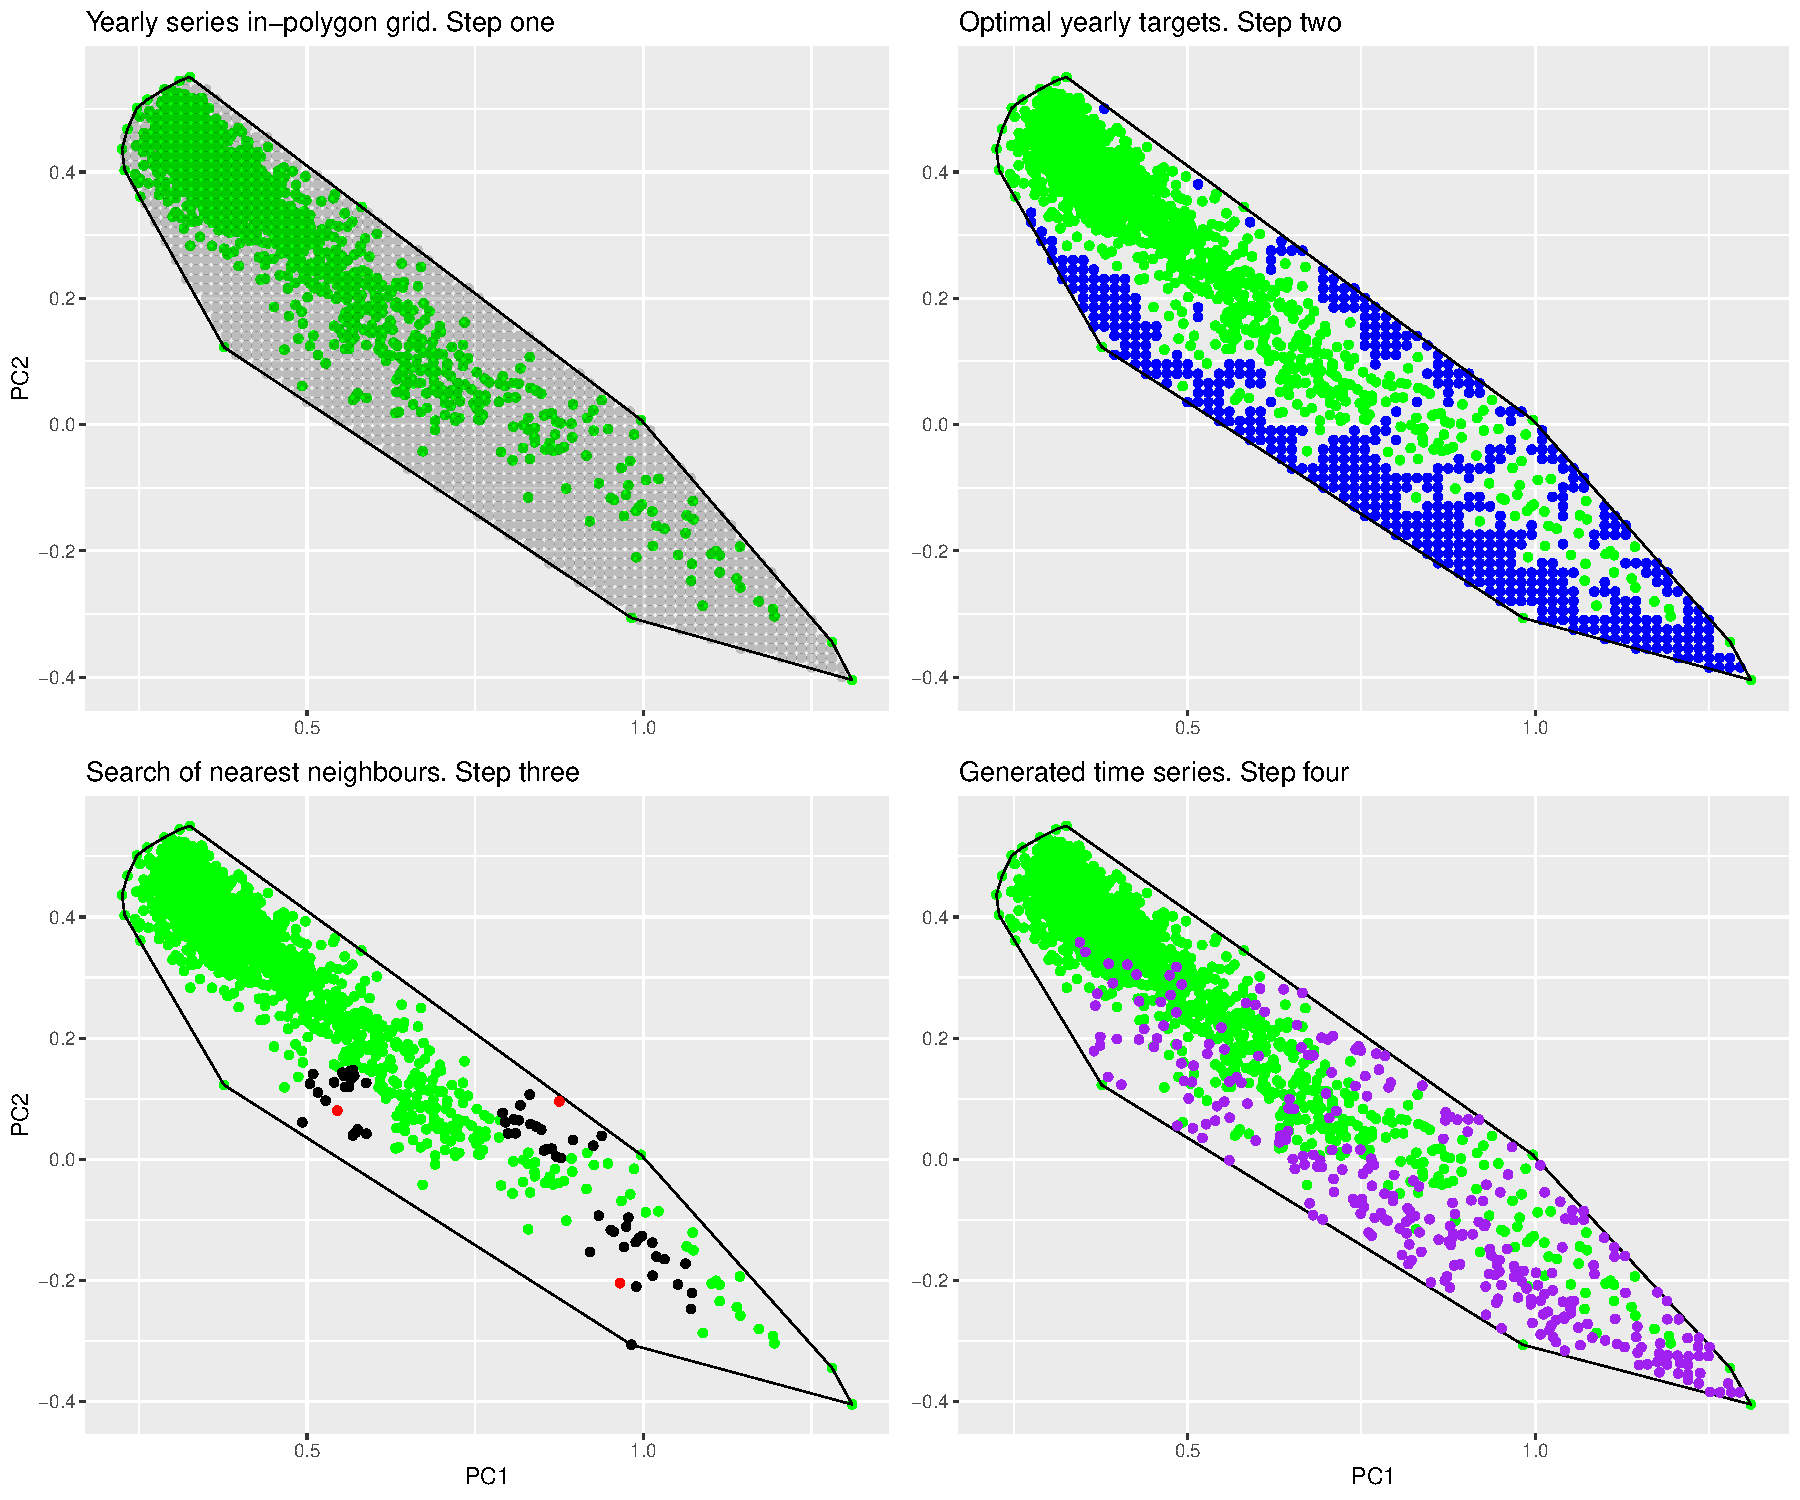
\includegraphics[width = 0.8\linewidth]{slides/generation_grid.pdf}
\end{center}
\end{frame}

\begin{frame}
\frametitle{Generated example}

\begin{center}
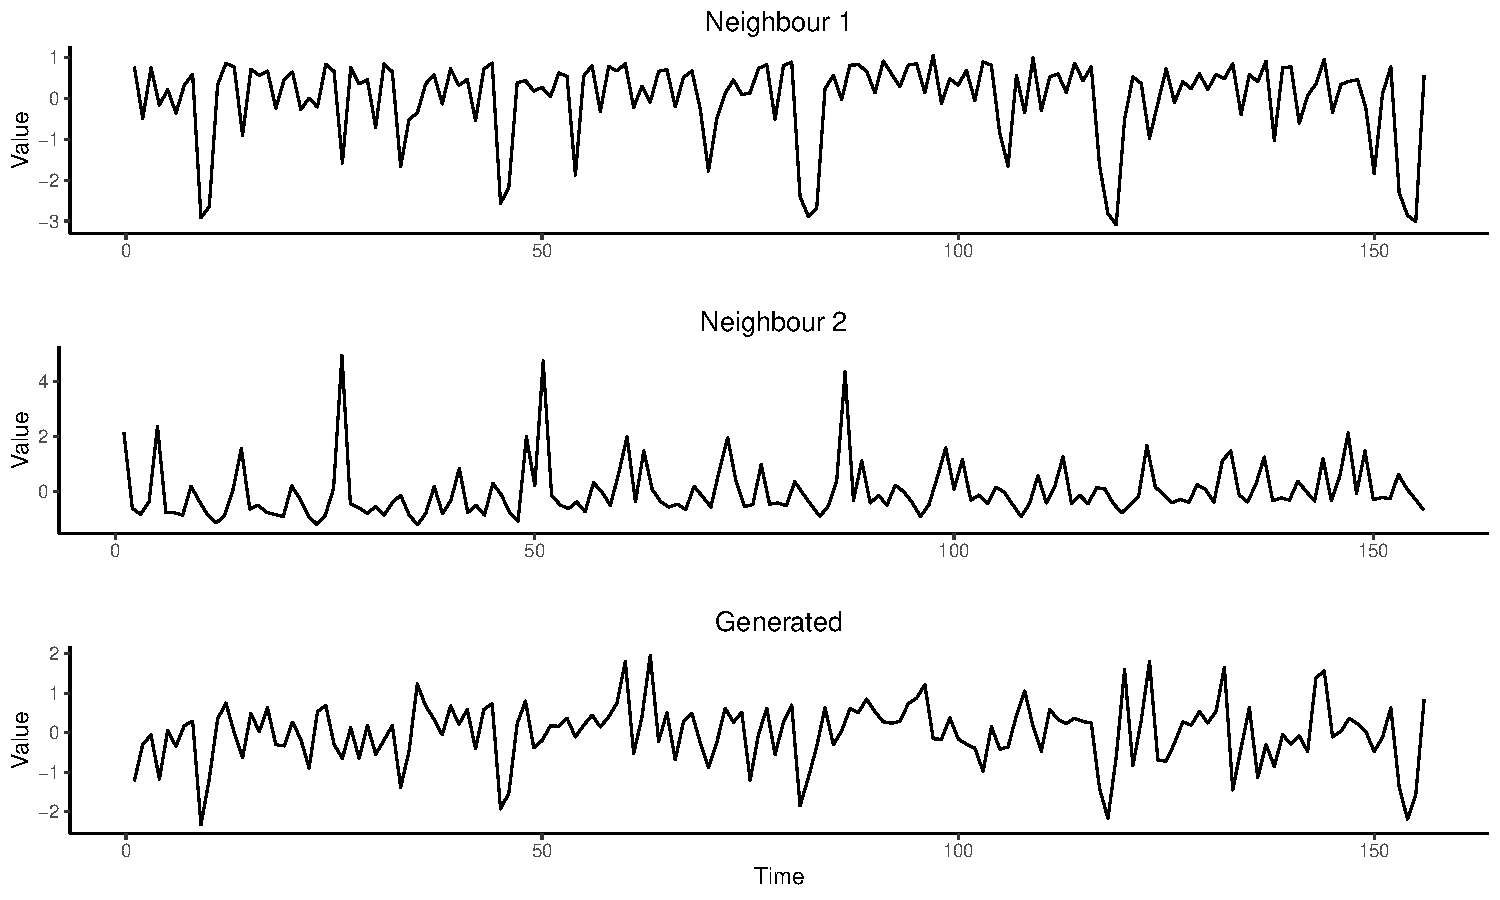
\includegraphics[width = 0.8\linewidth]{slides/gen_and_neighbours.pdf}
\end{center}
\end{frame}

\begin{frame}
\frametitle{Optimization process}

\begin{center}
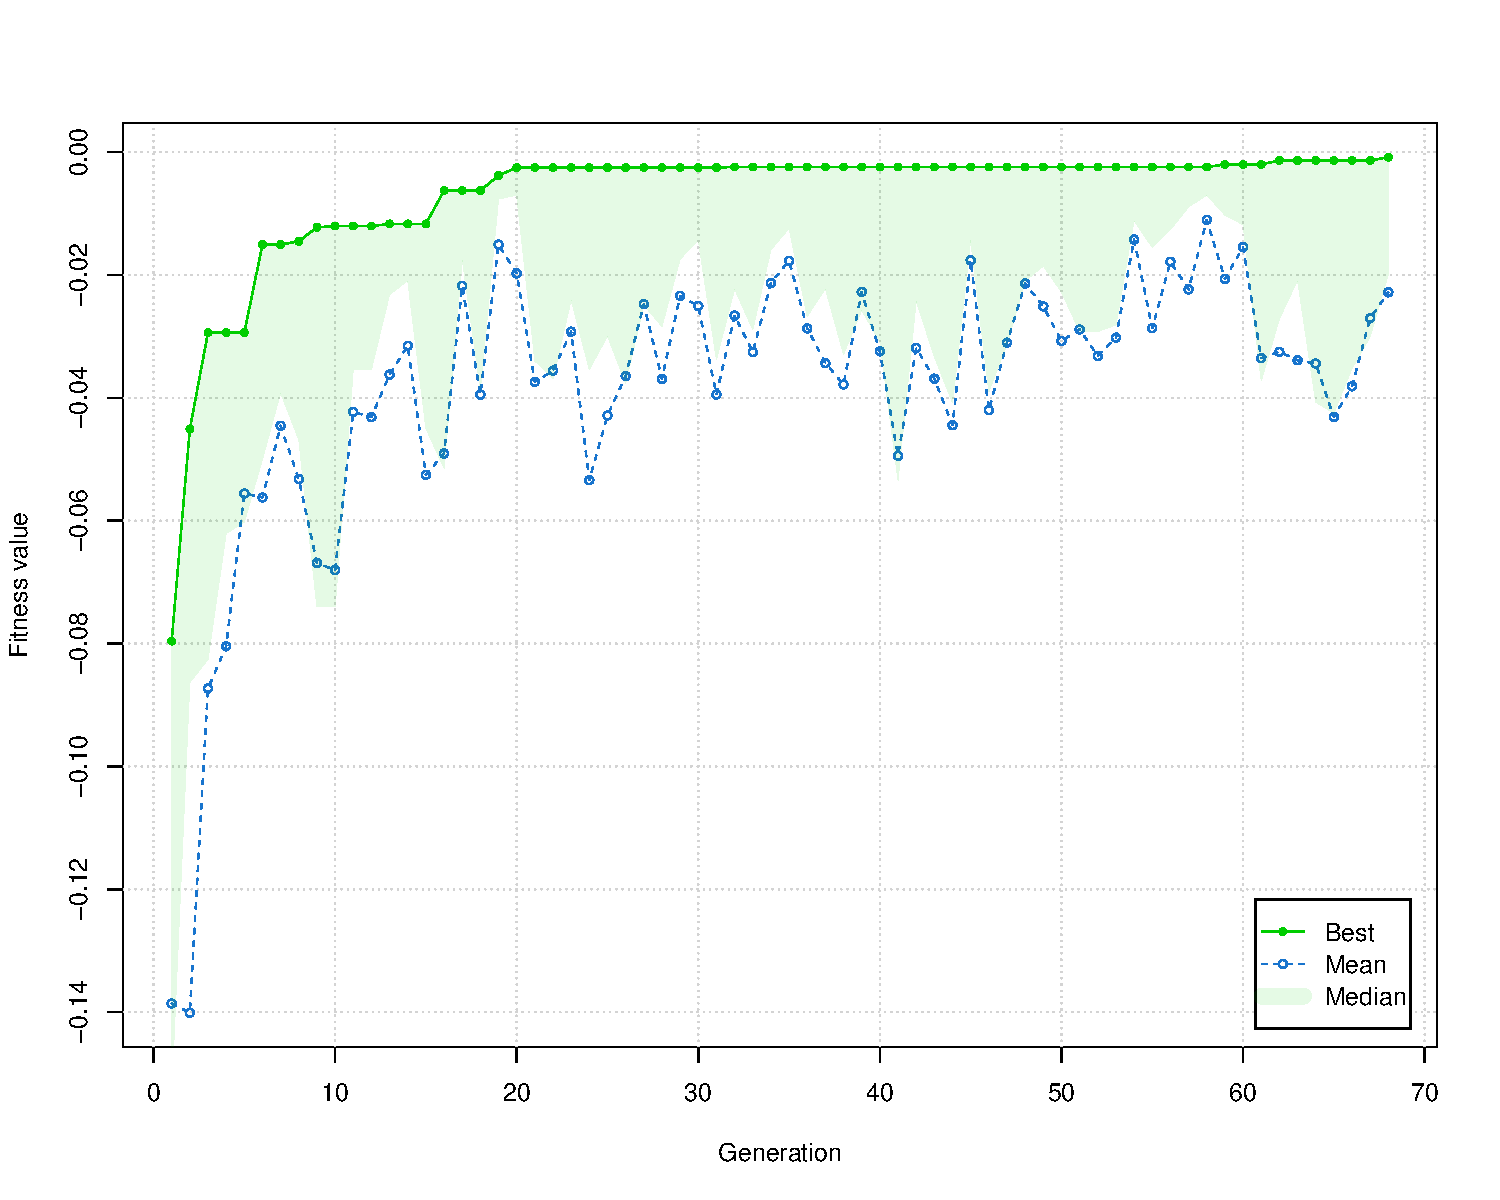
\includegraphics[width = 0.8\linewidth]{slides/optim.pdf}
\end{center}
\end{frame}

\begin{frame}
\frametitle{All generated series}

\begin{center}
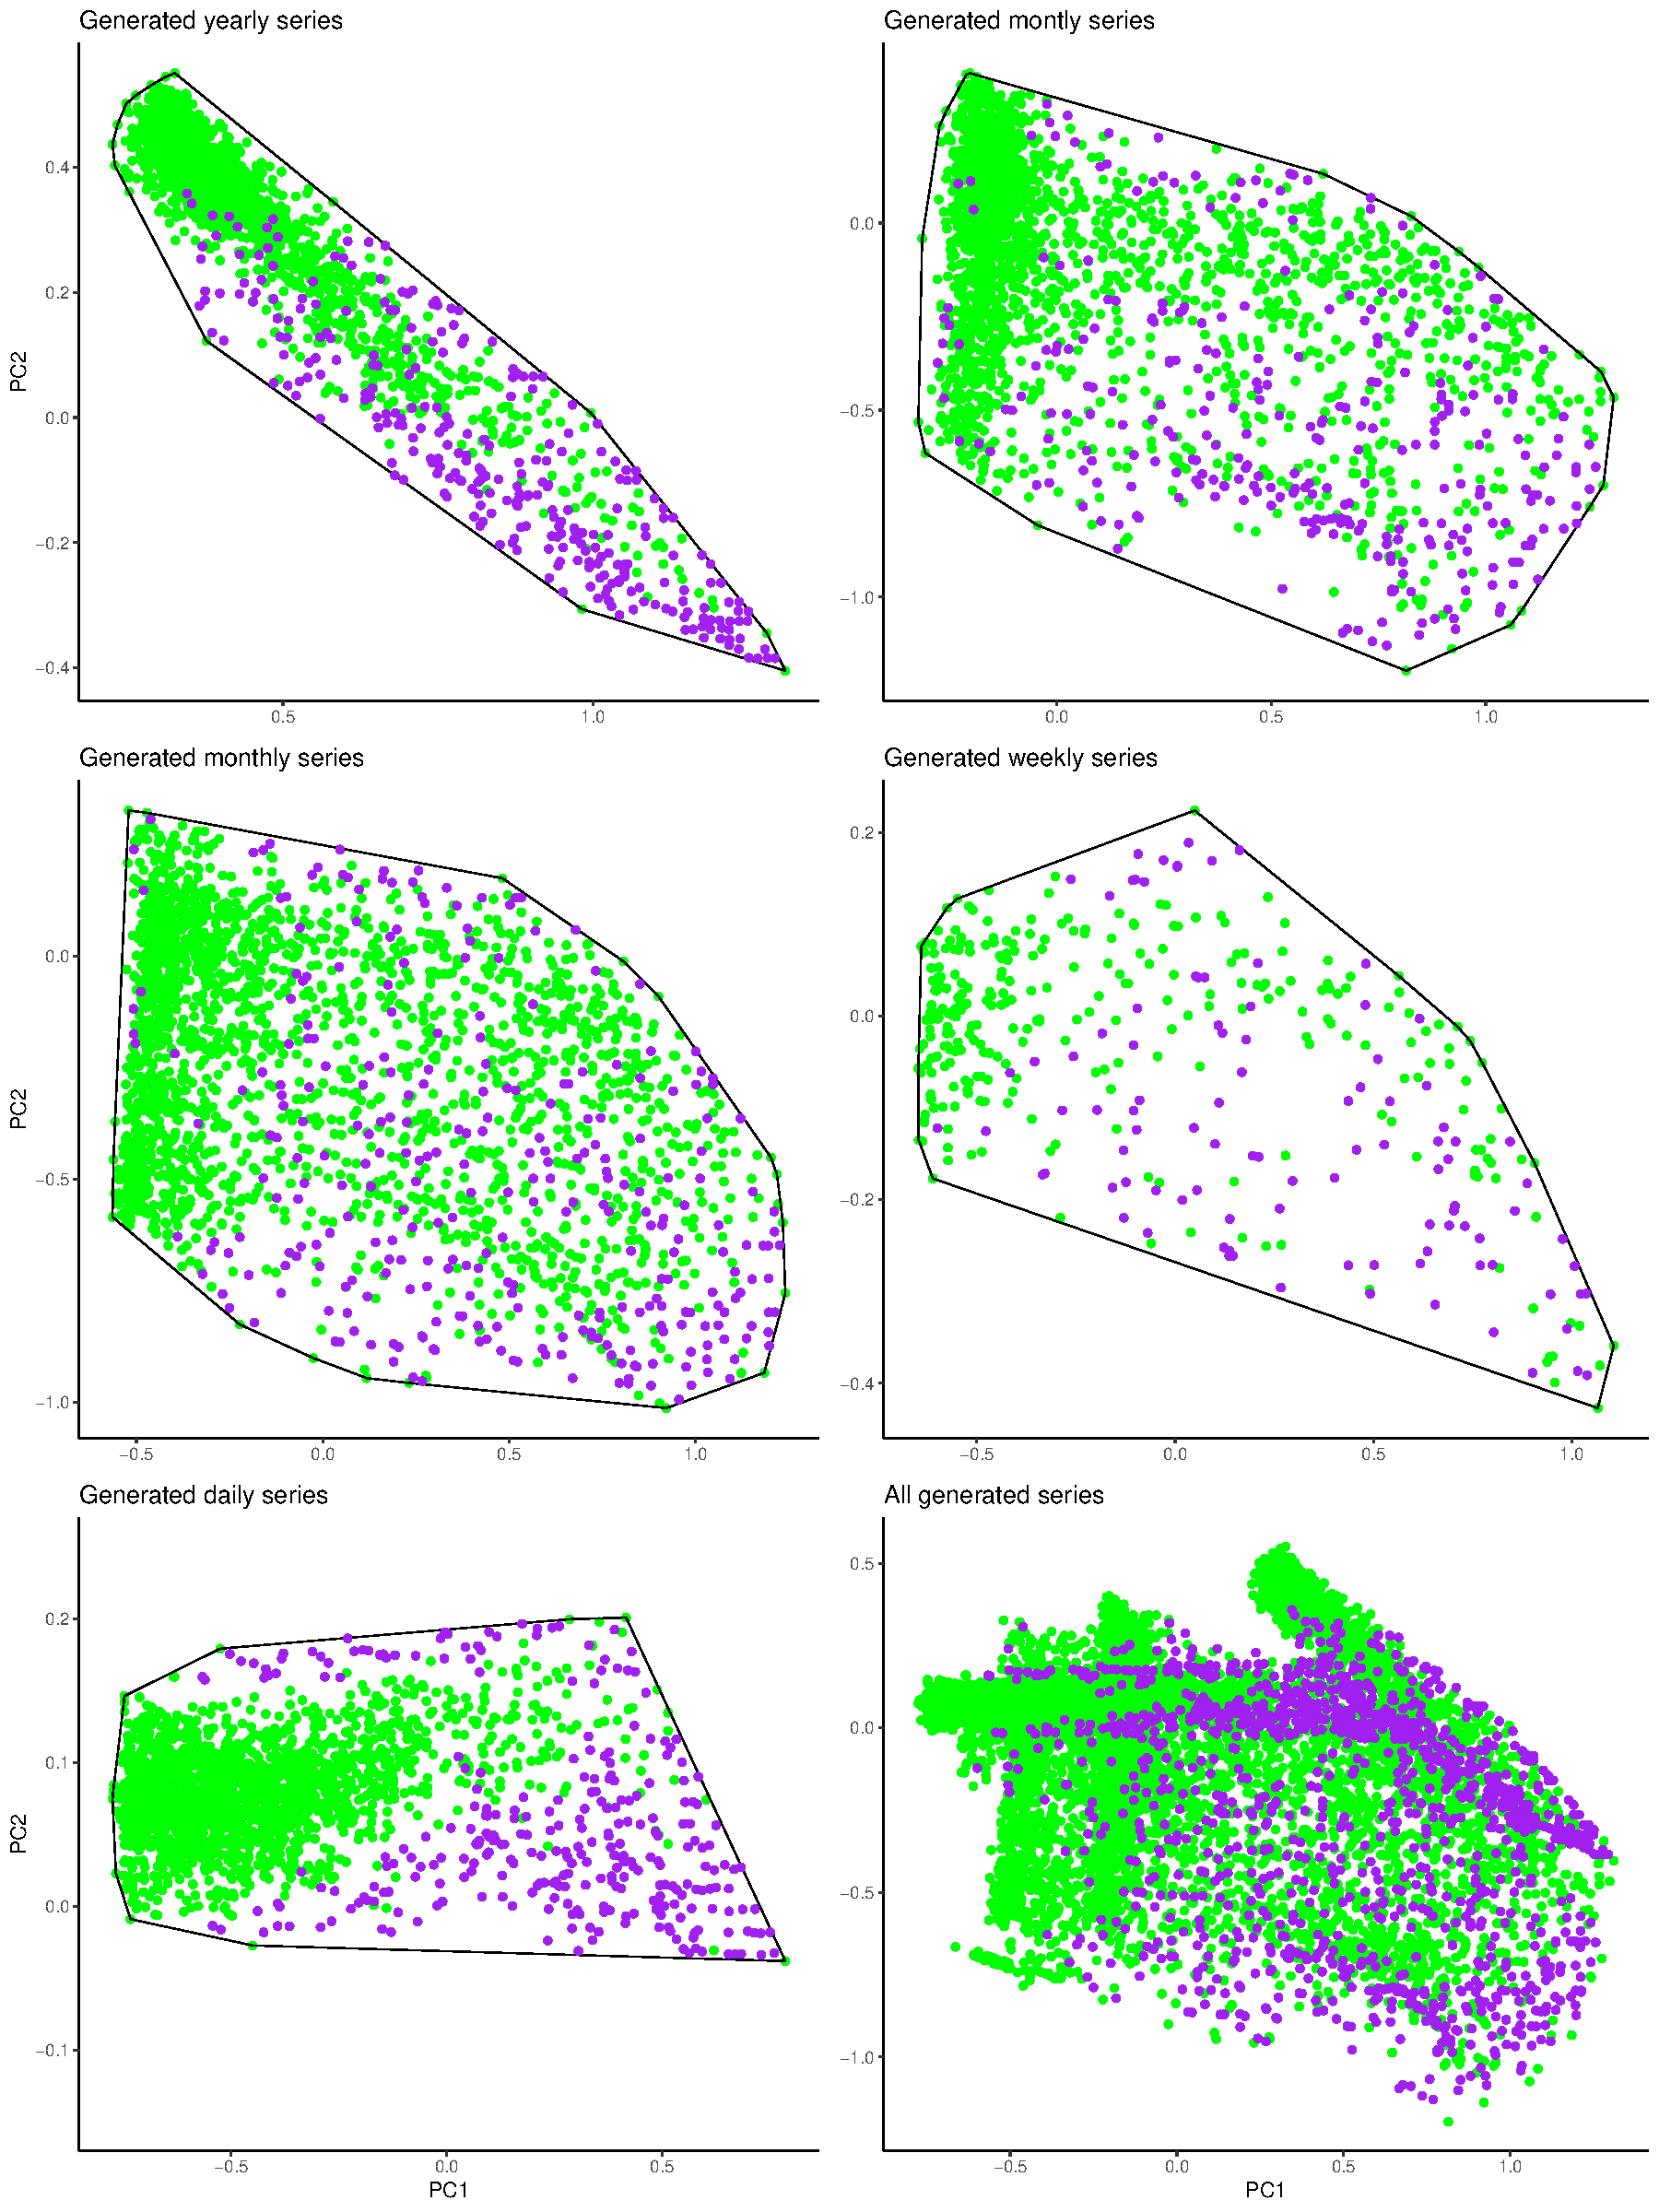
\includegraphics[width = 0.5\linewidth]{slides/all_gen.pdf}
\end{center}
\end{frame}


\begin{frame}
\frametitle{SMAPE of each model}

\begin{figure}
	\animategraphics[autoplay,controls,loop,scale=1,width=0.8\textwidth]{1}{slides/image}{1}{9}
\end{figure}
\end{frame}



\begin{frame}
\frametitle{Most acceptable model}
\begin{table}[]
\resizebox{\textwidth}{!}{%
\begin{tabular}{|
>{\columncolor[HTML]{91FF91}}l |
>{\columncolor[HTML]{FFFFFF}}l |
>{\columncolor[HTML]{FFFFFF}}l |
>{\columncolor[HTML]{FFFFFF}}l |
>{\columncolor[HTML]{FFFFFF}}l |
>{\columncolor[HTML]{FFFFFF}}l |}
\hline
\textbf{Model\textbackslash{}Class} & \cellcolor[HTML]{91FF91}\textbf{Yearly} & \cellcolor[HTML]{91FF91}\textbf{Quarterly} & \cellcolor[HTML]{91FF91}\textbf{Monthly} & \cellcolor[HTML]{91FF91}\textbf{Weekly} & \cellcolor[HTML]{91FF91}\textbf{Daily} \\ \hline
\textbf{Naive} & 204 | 9\% & 161 | 7\% & 112 | 5\% & 39 | 10\% & 90   | 4\% \\ \hline
\textbf{Seasonal Naive} & -- & 232 |10\% & 266 | 12\% & 39 | 10\% & 230 | 10\% \\ \hline
\textbf{RW with drift} & 333 | 14\% & 339 | 15\% & 271 | 12\% & 75 | 19\% & 595 | 26\% \\ \hline
\textbf{SES} & 112 | 5\% & 89   | 3\% & 86   | 4\% & 19 | 5\% & 88   | 4\% \\ \hline
\textbf{ETS} & 311 | 14\% & 288 | 13\% & 328 | 14\% & 24 | 6\% & 56   | 2\% \\ \hline
\textbf{ARIMA} & 366 | 16\% & \cellcolor[HTML]{91FF91}443 | 19\% & \cellcolor[HTML]{91FF91}466 | 20\% & 57 | 15\% & 247 | 12\% \\ \hline
\textbf{Theta} & 166 | 7\% & 127 | 6\% & 100 | 4\% & 11 | 3\% & 152 | 7\% \\ \hline
\textbf{TBATS} & \cellcolor[HTML]{91FF91}444 | 19\% & 288 | 13\% & 323 | 14\% & 40 | 10\% & 181 | 8\% \\ \hline
\textbf{Neural net} & 348 | 15\% & 127 | 6\% & 345 | 15\% & \cellcolor[HTML]{91FF91}82 | 21\% & \cellcolor[HTML]{91FF91}655 | 29\% \\ \hline
\textbf{Total} & 2284 & 2297 & 2297 & 386 & 2294 \\ \hline
\end{tabular}%
}
\end{table}
\end{frame}



\begin{frame}
\frametitle{Minimal SMAPE}
\begin{table}[]
\resizebox{\textwidth}{!}{%
\begin{tabular}{|l|l|l|l|l|l|l|l|l|l|l|}
\hline
\rowcolor[HTML]{91FF91} 
\textbf{Model\textbackslash{}Class} & \multicolumn{2}{l|}{\cellcolor[HTML]{91FF91}\textbf{Yearly}} & \multicolumn{2}{l|}{\cellcolor[HTML]{91FF91}\textbf{Quarterly}} & \multicolumn{2}{l|}{\cellcolor[HTML]{91FF91}\textbf{Monthly}} & \multicolumn{2}{l|}{\cellcolor[HTML]{91FF91}\textbf{Weekly}} & \multicolumn{2}{l|}{\cellcolor[HTML]{91FF91}\textbf{Daily}} \\ \hline
\rowcolor[HTML]{91FF91} 
\textbf{} & \textbf{Mean} & \textbf{Sd} & \textbf{Mean} & \textbf{Sd} & \textbf{Mean} & \textbf{Sd} & \textbf{Mean} & \textbf{Sd} & \textbf{Mean} & \textbf{Sd} \\ \hline
\rowcolor[HTML]{FFFFFF} 
\cellcolor[HTML]{91FF91}\textbf{Naive} & 0.732 & 0.637 & 0.469 & 0.467 & 0.541 & 0.418 & 0.533 & 0.417 & 0.550 & 0.540 \\ \hline
\rowcolor[HTML]{FFFFFF} 
\cellcolor[HTML]{91FF91}\textbf{Seasonal Naive} & -- & -- & 0.646 & 0.482 & 0.615 & 0.452 & 0.759 & 0.541 & 0.838 & 0.566 \\ \hline
\rowcolor[HTML]{FFFFFF} 
\cellcolor[HTML]{91FF91}\textbf{RW with drift} & 0.248 & 0.334 & 0.320 & 0.301 & 0.452 & 0.420 & 0.510 & 0.394 & 0.337 & 0.310 \\ \hline
\rowcolor[HTML]{FFFFFF} 
\cellcolor[HTML]{91FF91}\textbf{SES} & 0.369 & 0.482 & 0.341 & 0.339 & 0.462 & 0.422 & 0.441 & 0.467 & 0.349 & 0.421 \\ \hline
\rowcolor[HTML]{91FF91} 
\textbf{ETS} & 0.126 & 0.173 & 0.301 & 0.326 & \cellcolor[HTML]{FFFFFF}0.410 & \cellcolor[HTML]{FFFFFF}0.399 & 0.298 & 0.382 & 0.286 & 0.314 \\ \hline
\rowcolor[HTML]{FFFFFF} 
\cellcolor[HTML]{91FF91}\textbf{ARIMA} & 0.238 & 0.374 & 0.309 & 0.326 & \cellcolor[HTML]{91FF91}0.408 & \cellcolor[HTML]{91FF91}0.383 & 0.412 & 0.372 & 0.388 & 0.420 \\ \hline
\rowcolor[HTML]{FFFFFF} 
\cellcolor[HTML]{91FF91}\textbf{Theta} & 0.406 & 0.500 & 0.639 & 0.501 & 0.729 & 0.511 & 0.730 & 0.498 & 0.784 & 0.618 \\ \hline
\rowcolor[HTML]{FFFFFF} 
\cellcolor[HTML]{91FF91}\textbf{TBATS} & 0.233 & 0.343 & 0.312 & 0.358 & 0.438 & 0.429 & 0.424 & 0.437 & 0.486 & 0.459 \\ \hline
\rowcolor[HTML]{FFFFFF} 
\cellcolor[HTML]{91FF91}\textbf{Neural Net} & 0.454 & 0.511 & 0.493 & 0.430 & 0.509 & 0.425 & 0.683 & 0.473 & 0.605 & 0.474 \\ \hline
\end{tabular}%
}
\end{table}
\end{frame}

\begin{frame}
\frametitle{Thank you!}

\begin{center}

\includegraphics[width = 0.5\linewidth]{slides/poiss.jpg}
\end{center}
\end{frame}

% La première grande partie: introduction du sujet

\end{document}


